% Created 2024-02-29 Thu 11:50
% Intended LaTeX compiler: pdflatex
\documentclass[11pt]{article}
\usepackage[utf8]{inputenc}
\usepackage[T1]{fontenc}
\usepackage{graphicx}
\usepackage{longtable}
\usepackage{wrapfig}
\usepackage{rotating}
\usepackage[normalem]{ulem}
\usepackage{amsmath}
\usepackage{amssymb}
\usepackage{capt-of}
\usepackage{hyperref}
\hypersetup{colorlinks=true, allcolors=blue} \usepackage{titlesec} \usepackage{geometry} \geometry{margin=1.2in} \usepackage{minted} \newcommand{\sectionbreak}{\clearpage} \usepackage{graphicx} \usepackage{changepage} \usepackage{inconsolata}
\author{Matthew}
\date{\today}
\title{}
\hypersetup{
 pdfauthor={Matthew},
 pdftitle={},
 pdfkeywords={},
 pdfsubject={},
 pdfcreator={Emacs 28.3 (Org mode 9.7)}, 
 pdflang={English}}
\begin{document}

\begin{LATEX}
\begin{titlepage}

  \centering
  {\Large\bfseries Big Data Assignment 1 \par}
  \vspace{0.5cm}

  {\large KFWJOR001 MRCGAB004 WHLJOS001 CRGMAT002\par}
  \vspace{0.5cm}

  {\large March 1, 2024\par}

  \vspace{2cm}
  
\includegraphics[width=0.4\textwidth]{mongo.png}
  
\includegraphics[width=0.4\textwidth]{uct.png}
\end{titlepage}
\tableofcontents
\end{LATEX}
\pagebreak
\section{Find or Create a Suitable Data Set}
\label{sec:org395ac93}
\subsection{Data Set Explanation}
\label{sec:orgf5b45a1}
Link to the dataset: \url{https://github.com/zygmuntz/goodbooks-10k}\\
\linebreak
The dataset includes data from an online book review platform (\url{https://goodreads.com/}). It includes information about the books, users, book tags, and book rating scores. The dataset initially contained multiple csv files. This dataset was chosen as its ideal for a MongoDB database due to its semi-structured nature and nested data, which is particularly useful for storing ratings and book tags. \\
\linebreak
\textbf{Dataset Content}:
\begin{itemize}
\item \textbf{books.csv}: Each entry represents a book with a unique \texttt{book\_id}. There are multiple data fields for a book:
\begin{itemize}
\item \textbf{\texttt{book\_id}, \texttt{goodreads\_book\_id}, \texttt{best\_book\_id}, \texttt{work\_id}}: Unique id’s representing a book, each with a different purpose. We only used \texttt{book\_id} and \texttt{goodreads\_book\_id} as they’re used to link books to user \texttt{ratings} and user \texttt{to\_read} lists.
\item \textbf{\texttt{ratings\_1}, \texttt{ratings\_2}, …}: Number of user ratings by rating value. eg. \texttt{ratings\_1} represents the number of 1 star ratings given to that book.
\item The rest of the fields are self explanatory but include info relating to authors, title, release date, and isbn number.
\end{itemize}
\item \textbf{ratings.csv}: Each entry is a \texttt{user\_id} to \texttt{book\_id} mapping with a rating.
\begin{itemize}
\item \textbf{\texttt{book\_tags.csv}}: Each entry is a \texttt{book\_id} to \texttt{tag\_id} mapping.
\item \textbf{\texttt{tags.csv}}: Each entry is a tag\textsubscript{id} to \texttt{tag\_name} mapping.
\item \textbf{\texttt{to\_read.csv}} : Each entry is a \texttt{user\_id} to \texttt{goodreads\_book\_id} mapping which represents a user adding a book to their \texttt{to\_read} list.
\end{itemize}
\end{itemize}
\subsection{Data Pre-Processing}
\label{sec:org72fecc5}
The data was processed such that the data was represented in JSON format with evidence of nested objects so that we could demonstrate the capabilities of MongoDB.\\
\linebreak
Here is a quick outline on how we processed the data to create JSON files:\\
Libraries used: \texttt{Pandas}, \texttt{PyArrow}, \texttt{Faker}\\
\linebreak
\texttt{Pandas} was used to load the csv files into dataframes where we merged data and applied \texttt{group by} aggregate functions to obtain lists of data objects per a unique entry id. This was useful, for example, when we obtained a list of tags per \texttt{book\_id}.\\
\linebreak
\texttt{Faker} was used to generate random usernames for each id that were then written to \texttt{user\_data.csv}. The \texttt{dataframes} were then converted into JSON files.\\
\linebreak
All data pre-processing code is in the data-processing directory but the output JSON files are included in the final submission.
\section{Design a MongoDB Database}
\label{sec:orgea2ceda}
Both Collection Schemas were designed by creating hand-made JSON example objects. Each of these objects shows what a document in the DB would look like. Underneath each JSON example, we have included a diagram which represents the example's nesting visually.
\subsection{Collection 1 - \texttt{books}}
\label{sec:orgfeac505}

\paragraph{JSON example} \small
\begin{minted}[]{js}
{
    "book_id": "98",
    "isbn": "1401359604",
    "isbn13": "9781401359610.0",
    "authors": [
        "Plum Sykes"
    ],
    "original_publication_year": 2004,
    "title": "Bergdorf Blondes",
    "language_code": "en-US",
    "average_rating": 3.26,
    "ratings_count": 23795,
    "total_ratings": {
        "ratings_1": 2020,
        "ratings_2": 4428,
        "ratings_3": 8669,
        "ratings_4": 6144,
        "ratings_5": 4561
    },
    "image_url": "https://s.gr-assets.com/assets/nophoto/book/111x148-bcc042a9c91a29c1d680899eff700a03.png",
    "tags": [
        {
            "tag_id": 11743,
            "tag_name": "fiction"
        },
        {
            "tag_id": 8717,
            "tag_name": "currently-reading"
        },
        {
            "tag_id": 8055,
            "tag_name": "contemporary"
        }
    ],
    "ratings": [
        {
            "user": {
                "user_id": 237,
                "user_name": "David Smith"
            },
            "rating": 1
        },
        {
            "user": {
                "user_id": 364,
                "user_name": "Christina Calderon"
            },
            "rating": 1
        },
        {
            "user": {
                "user_id": 399,
                "user_name": "Stephen Pugh"
            },
            "rating": 2
        }
    ]
}
\end{minted}

\newgeometry{margin=0in}
\begin{center}
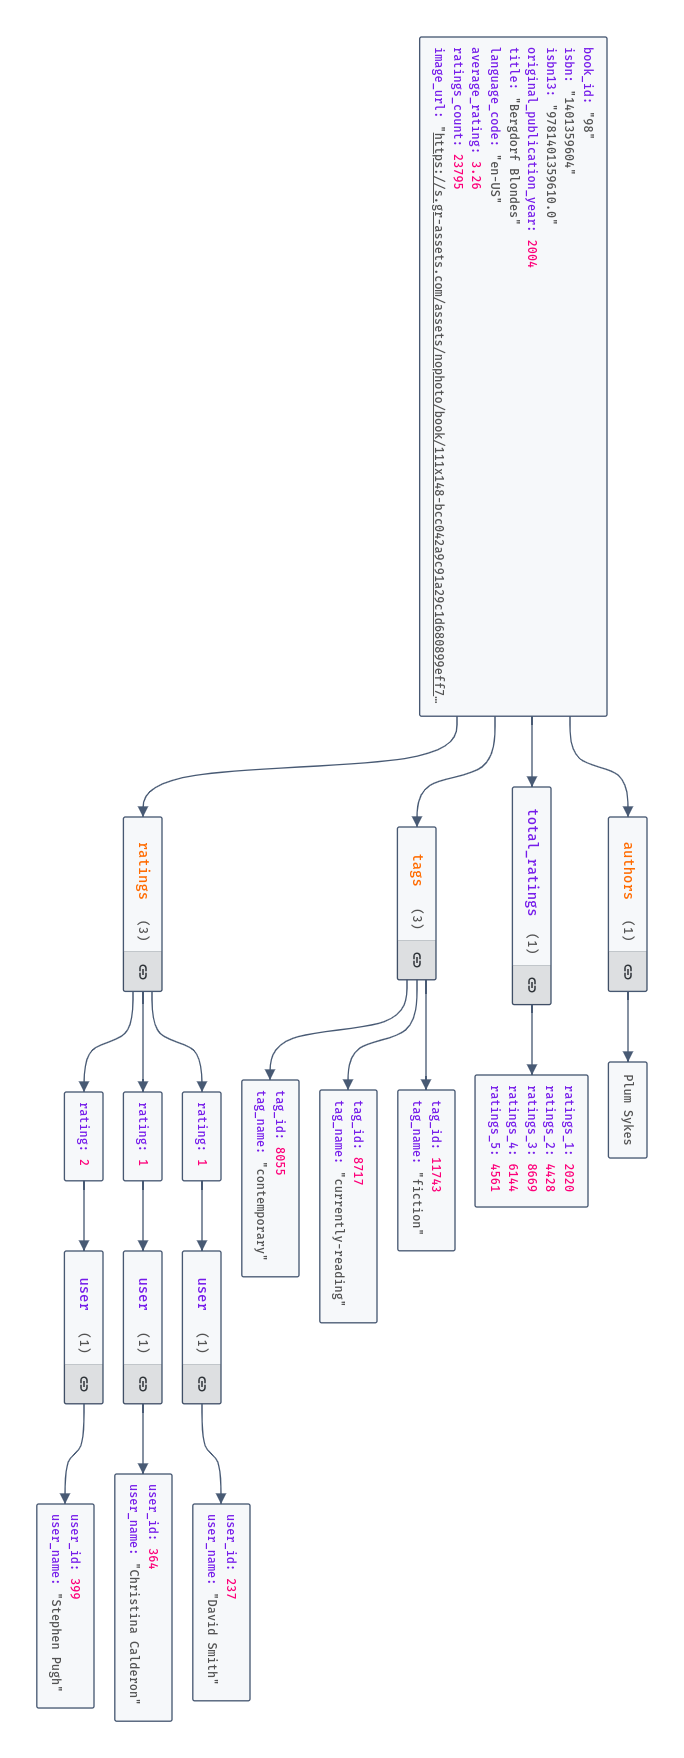
\includegraphics[height=1.2\textwidth]{Collection1Rotate.png}
\end{center}
\restoregeometry
\subsection{Collection 2 - \texttt{users}}
\label{sec:org8287b57}

\begin{minted}[]{js}
{
    "user_id": 1,
    "user_name": "Mary Martinez",
    "ratings": [
        {
            "book": {
                "book_id": 47,
                "authors": [
                    "Markus Zusak"
                ],
                "title": "The Book Thief",
                "isbn": "375831002",
                "isbn13": 9780375831000.0,
                "language_code": "eng",
                "average_rating": 4.36,
                "ratings_count": 1159741,
                "image_url": "https://images.gr-assets.com/books/1390053681m/19063.jpg",
                "tags": [
                    {
                        "tag_id": 11557,
                        "tag_name": "favorites"
                    },
                    {
                        "tag_id": 30574,
                        "tag_name": "to-read"
                    },
                    {
                        "tag_id": 14487,
                        "tag_name": "historical-fiction"
                    },
                    {
                        "tag_id": 11743,
                        "tag_name": "fiction"
                    },
                    {
                        "tag_id": 33114,
                        "tag_name": "young-adult"
                    }
                ]
            },
            "rating": 3
        }
    ],
    "to_read": [
        {
            "book": {
                "book_id": 112,
                "authors": [
                    "Jojo Moyes"
                ],
                "title": "Me Before You",
                "isbn": "670026603",
                "isbn13": 9780670026610.0,
                "language_code": "eng",
                "average_rating": 4.27,
                "ratings_count": 587647,
                "image_url": "https://images.gr-assets.com/books/1357108762m/15507958.jpg",
                "tags": [
                    {
                        "tag_id": 30574,
                        "tag_name": "to-read"
                    },
                    {
                        "tag_id": 11557,
                        "tag_name": "favorites"
                    },
                    {
                        "tag_id": 17213,
                        "tag_name": "kindle"
                    },
                    {
                        "tag_id": 26138,
                        "tag_name": "romance"
                    },
                    {
                        "tag_id": 3389,
                        "tag_name": "audiobook"
                    }
                ]
            }
        }
    ]
}
\end{minted}

\newgeometry{margin=0in}
\begin{center}
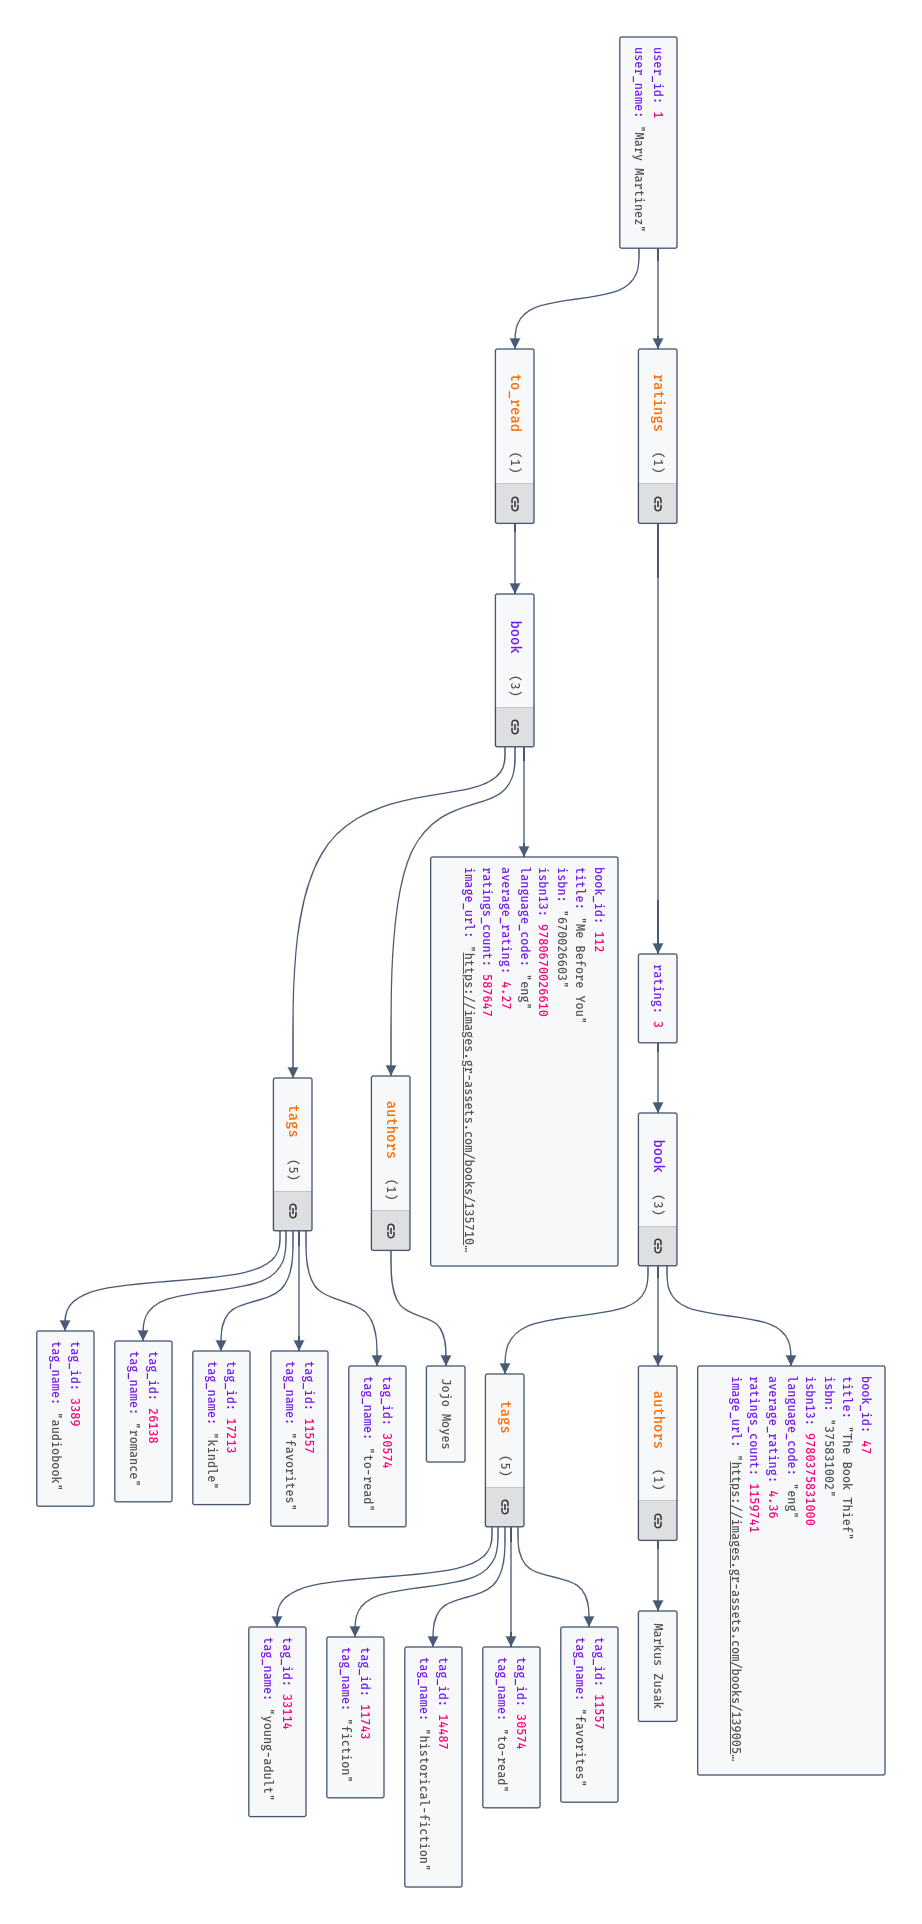
\includegraphics[height=1.2\textwidth]{Collection2Rotate.png}
\end{center}
\restoregeometry
\subsection{Explanation and Justification}
\label{sec:org6011510}
The data in CSV format emulates the functionality of a relational database. Many of the fields have foreign keys that point to elements in the other CSV files. Document store database favour efficiency over consistency, thus, we have nested a copy of the relevant object where the value would have otherwise been a foreign key. The process by how this was achieved was highlighted in ``\hyperref[sec:org72fecc5]{Data Pre-Processing}''.

The data was seeded into the following 2 collections:
\begin{itemize}
\item \texttt{books}
\item \texttt{users}\\
\end{itemize}
\linebreak
\subsubsection{Books}
\label{sec:orgcde58f5}
The \texttt{books} collection roughly followed the format of \texttt{books.csv} (outlined in ``\hyperref[sec:orgf5b45a1]{Data Set Explanation}'') with some modifications. We omitted unnecessary information and altered the names of some of the properties to make their semantic meaning clearer. As a result each book document includes:
\begin{itemize}
\item General information about the book (\texttt{title}, \texttt{author}, \texttt{original\_publication\_year}, etc.).
\item Aggregated rating values (\texttt{average\_rating}, \texttt{total\_ratings}, \texttt{ratings\_counts}).
\item A \texttt{ratings} list
\begin{itemize}
\item Each element represents a \texttt{user}'s review of that book. It includes the \texttt{user}'s basic information and the assigned \texttt{rating} score.
\end{itemize}
\item A \texttt{tags} list. Each tag represents a genre or category the book belongs to.\\
\end{itemize}
\linebreak
The most significant element of our design was the aforementioned nesting. Rather than store a separate \texttt{tags} collection, all the tags associated with the book are stored as a list of objects. The same is true for \texttt{ratings}, which is a list of rating objects.\\
\linebreak
Use case examples:\\
\begin{itemize}
\item Collection of books: Querying to see the average rating of a book and the distribution of ratings of a particular book
\end{itemize}
\subsubsection{Users}
\label{sec:orga31f734}
Unlike \texttt{books}, the \texttt{users} collection does not directly correspond to a csv file. Instead, \texttt{users} was created by combining data from \texttt{ratings.csv}, \texttt{to\_read.csv}, and \texttt{books.csv}. We chose to create the user collection in order to demonstrate the importance of collection design with regards to query efficiency. While the \texttt{users} contains a lot of duplicate data from \texttt{books}, it does so in a way that places information about the users at the top of the nesting hierarchy. This means that data about individual users can be obtained without performing expensive joins. The chosen collection design allows one to access, store and perform analytics from the perspective of the user. Each document in the \texttt{users} collection includes the following:
\begin{itemize}
\item A \texttt{user\_id} and \texttt{user\_name} (randomly generated, as explained in ``\hyperref[sec:org72fecc5]{Data Pre-Processing}'').
\item A \texttt{ratings} list:
\begin{itemize}
\item Each element represents a score that the user has given to a book.
\item The element includes a \texttt{book} object and a given \texttt{rating} score.
\item The nested \texttt{book} object includes all high-level data about that book, as would be found in the \texttt{books} collection.
\end{itemize}
\item A \texttt{to\_read} list.
\begin{itemize}
\item Each element represents a book that the user has added to their \texttt{to\_read} list (ie. plans to read that book).
\item The element is represented as a \texttt{book} object that is identical in structure to those represented in the \texttt{ratings} list.\\
\end{itemize}
\end{itemize}
\linebreak
Use case examples:\\
        Collection of users: what books user X wants to read.
\section{Create and Load This MongoDB Database}
\label{sec:org0337c65}
\subsection{Load the Database}
\label{sec:org88d3fe5}
The process of creating and loading the database was significantly simplified on account of the fact that we had already \hyperref[sec:org72fecc5]{Pre-Processed} the data into JSON format. For each collection, a shell command is called to seed the JSON data into their associated collections. The creation of the database is implicit ie. inserting data into the non-existent database leads to its creation. The commands use \texttt{mongoimport}, a CLI tool designed for extracting data from plain-text formats (eg. JSON) and inserting them into MongoDB databases.
\subsubsection{Books Collection}
\label{sec:org51e4dd6}
\begin{minted}[]{bash}
mongoimport --db bookstore --collection books --file mongo-seed/books.json --jsonArray
\end{minted}
\subsubsection{Users Collection}
\label{sec:org2878ab4}
\begin{minted}[]{bash}
mongoimport --db bookstore --collection users --file mongo-seed/users.json --jsonArray
\end{minted}
\subsection{Testing}
\label{sec:org1c63bb6}
The shell commands were tested and the output has been annotated on the following page:
\newgeometry{margin=0.1in}
\begin{center}
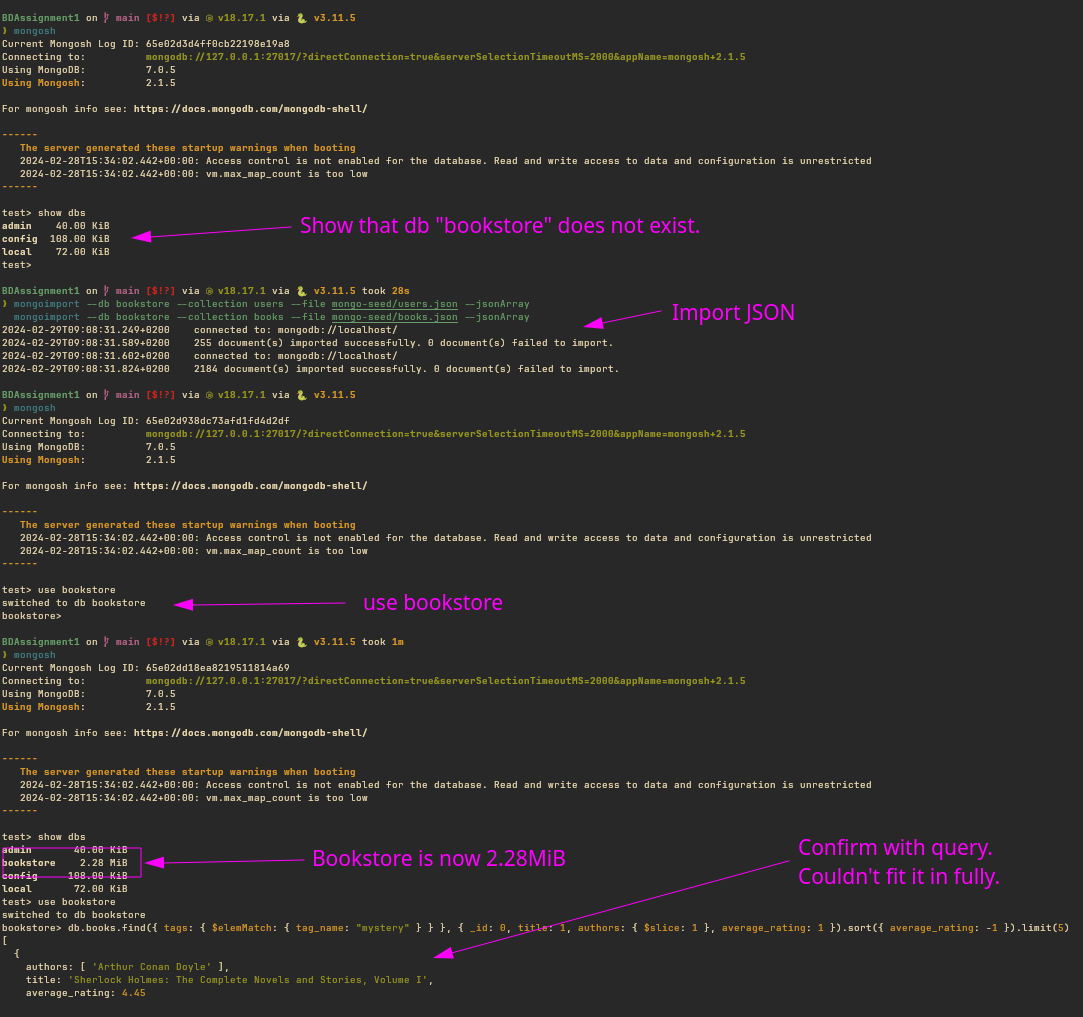
\includegraphics[width=1\textwidth]{q3.png}
\end{center}
\restoregeometry
\section{Discuss the Relative Benefits and Disadvantages of MongoDB}
\label{sec:org7c5b9c7}
\subsection{MongoDB (Document Store)}
\label{sec:orgf123549}
MongoDB is a document store database. Document store databases favour low retrieval latency and efficiency over consistency and functionality (expressiveness) when compared with relational databases. MongoDB is flexible: it fascilitates incremental schema modification as the schema is not rigidly defined. This can improve development velocity and account for changing stakeholder requirements.\\
\linebreak
MongoDB is highly scalable and will be efficient with the ever increasing addition of books being published. MongoDB meets a good middle-ground when compared with other NoSQL databases. It is fascilitates nested data and objects and allows querying on those objects without being overly strict or complex. Each Book and User is able to store all necessary information while allow for performant data retrieval without the overhead of complex joins.\\
\linebreak
The disadvantages of using a MongoDB is that there is a high degree of duplication and redundant data. This means that storing and transferring all of this data is computationally expensive. Secondly, inserting and updating data can be much more expensive than a relational database on account of the necessity to make updates in multiple places (due to the duplication). However, data about books is unlikely to change frequently (as the book has already been published) and thus this downside is heavily mitigated in the chosen example.

\begin{itemize}
\item \textbf{Benefits} (When compared with relational): Scalable, schema-free design, data-access performance
\item \textbf{Disadvantages} (When compared with relational): Duplication, high storage use, slow modification, poor query expressiveness (functionality)
\item \textbf{Role in polyglot persistence}:
\begin{itemize}
\item A future polyglot design could store data that is high in volume but does not change frequently inside a document store db.
\item Books do not change frequently so the information about the books could be stored in the document store while users and ratings could be stored in other databases.
\item User telemetry could also be stored as in a document store database as it is high volume with very infrequent modification
\end{itemize}
\end{itemize}
\subsection{Graph}
\label{sec:orga893f53}
Graph based databases allow for expressive and performant relationship representation and would be ideal for relationship related queries. Each relationship can be given properties that qualitatively describe that relationship. This is ideal for data where the relationships to other data is the primary provider of utility (eg. a knowledge graph), as opposed to the hierarchical categorisation (as is the case in MongoDB and relational databases). The chosen dataset is intrinsically hierarchical and it thus be a poor choice for graph DBs. The dataset would not leverage the benefits of a graph DB and would miss out on the well-fitted the benefits of MongoDB, namely schema flexibility, performance, and scalability, and simplicity.
\begin{itemize}
\item \textbf{Benefits}: Efficient modelling of highly inter-linked data, Query expressiveness (functionality), Great relationship representation (for which it is scalable and performant)
\item \textbf{Disavantages}: Unnecessary complexity, poor modelling of hierarchical/structured data
\item \textbf{Role in polyglot persistence}:
\begin{itemize}
\item A future polyglot design could include a graph database that models the relationship books have to each other.
\item Each book could have an outgoing edge to related books with a descriptive tag that describes their relationship strength and type.
\item This would prove highly useful for the sites recommendation engine.
\end{itemize}
\end{itemize}
\subsection{Key-value}
\label{sec:org2690425}
Benefits:High performance, Simplicity, Flexible
Disadvantages: Limited query capabilities and Does not support complex data structures.
Role in polyglot persistence: It can store the current session data of users. Easy to keep track of users' sessions such as how long they were on the app.

Flexibility would be very important as it would allow us to store more complex session information about the user which can be used for processing later on to improve the users experience on the application.
Column-family
Column family databases could work well with the ‘good reads' dataset in calculating metrics and performing analytics, such as how many books are users reading and the total number of stars people rated individual books, how long people stay on the website, etc. The disadvantages are the queries one can perform are more basic and one cannot perform more complex queries beyond this.

Benefits: Compression of data, Scalable, fast to load queries, good for simple analytics
Disadvantages:limited querying capabilities, limited data modelling capabilities
Role in polyglot persistence: cannot think of any reason for its use on goodreads data storage. We would always have the same values for each object and so a columns family compression/efficiency would not be needed

Relational

Relational databases are great for keeping data consistent and for effectively maintaining the relationships of the data. The issue comes when we have too much data. Data analysis and operations are impacted substantially. it becomes inefficient with a very large (big) amount of data which is the issue one would run into with good-reads.

Benefits: Easy to use, accuracy, data integrity
Disadvantages:cost , physical storage, decrease in performance over time
Role in polyglot persistence:no function needed in this data but a good use case would be for keeping track of transactional data. Database is so large that one needs to use Nosql techniques to not be impacted by the size the relational database will create. We do not keep track of transactions as well so would not need the data integrity of a relational database
Hierarchical
Hierarchical databases are great for data with inherent hierarchies. Hierarchical databases would be great for fast lookup and to effectively store data. The issue is the data isn't inherently hierarchical and there are much more effective structures one could use to store the good reads data set.

Benefits:Fast data retrieval, efficient storage of data, predictable data structure,
Disadvantages:Limited flexibility, hard to maintain and update, limited interoperability.
Role in polyglot persistence: cannot think of any reason for its use on goodreads data storage.Our data is not hierarchical in structure and is flat and so there would be no need for a hierarchical data structure.
\end{document}
